\documentclass[12pt]{article}
\usepackage{geometry}
\geometry{letterpaper}
\usepackage[parfill]{parskip}
\usepackage{graphicx}
\usepackage{amssymb}
\usepackage{amsmath}
\usepackage{booktabs}
\usepackage{topcapt}
\usepackage{setspace}
\usepackage{xcolor}

\usepackage[T1]{fontenc}

%%%% TIKZ

\definecolor{s1}{RGB}{228, 26, 28}
\definecolor{s2}{RGB}{55, 126, 184}
\definecolor{s3}{RGB}{77, 175, 74}
\definecolor{s4}{RGB}{152, 78, 163}
\definecolor{s5}{RGB}{255, 127, 0}

\definecolor{p1}{RGB}{166, 97, 26}
\definecolor{p2}{RGB}{233, 194, 125}
\definecolor{p3}{RGB}{245, 245, 245}
\definecolor{p4}{RGB}{128, 205, 193}
\definecolor{p5}{RGB}{1, 133, 113}

\usepackage{pgfplots}
\usepackage{pgfplotstable}
\pgfplotsset{compat=newest}
\usepgfplotslibrary{groupplots}

\tikzset{
	every mark/.append style={scale=0.5},
	every axis grid/.append style = {color=black!40, dotted}
	}

\pgfplotscreateplotcyclelist{hc}{%
    s1,every mark/.append style={fill=s1},mark=*\\%
	s2,every mark/.append style={fill=s2},mark=*\\%
	s3,every mark/.append style={fill=s3},mark=*\\%
	s4,every mark/.append style={fill=s4},mark=*\\%
	s5,every mark/.append style={fill=s5},mark=*\\%
}

\pgfplotscreateplotcyclelist{pastel}{%
    p1!50!black,fill=p1\\%
	p2!50!black,fill=p2\\%
	p3!50!black,fill=p3\\%
	p4!50!black,fill=p4\\%
	p5!50!black,fill=p5\\%
}

\title{Functioning is predicted by trophic structure in complex ecosystems}
\author{Timoth\'ee Poisot\and Daniel Stouffer\and Dominique Gravel}
\date{WORKING PAPER}

\usepackage[doi=false,isbn=false,url=false]{biblatex}
\bibliography{/home/tpoisot/texmf/bibtex/bib/local/library.bib}

\begin{document}
\maketitle\doublespacing

\section{Introduction}

%% Complexity of food webs, need to find simple predictors
The complexity of natural ecological communities was qualified of
\emph{`baroque'} \parencite{holt_community_1997}, on account of the
multiplicity of ways in which two or more species can embed themselves in a
web of interactions. This prompted a series of studies of ``community
modules'', that is the interactions between three species, which were though
to be the right scale of observation to capture mechanisms underlying the
organization of more complex ecosystems. Recent research on species
interaction networks in general, and food webs in particular, aimed at making
sense of this complexity at a large scale, and render it manageable.
\textcite{berlow_simple_2009} showed that perturbations of one species rarely
spread farther than one or two of its closest neighbors, meaning that even in
highly complex networks, community modules are an appropriate scale at which
dynamical processes can be observed.

%% Challenges in linking structure to functioning

Establishing links between the structure and the dynamics of food webs is a
firmly established research agenda \parencite{Pascual2006}, and one which have
been taking prominence over the last few years so as to understand how trophic
downgrading will affect the maintenance of ecosystem services
\parencite{Estes2011}. Yet, our understanding of this relationship is scarce:
most research focused on the variations in biomass of species as a function of
their position in the food web \parencite{Williams2007,Berlow2009}, which is
still a very species-centric view. Most of our knowledge about the fact that
food web structure does affects the functioning of ecosystem comes from
analyses of networks of low complexity (i.e. discrete, well identified trophic
levels), and focused on extreme cases of connectance
\parencite[e.g.][]{Thebault2003,Thebault2007}. These studies emphasized that
functioning is driven by food web structure, but did not pinpoint a unifying
mechanism. In a recent contribution, we propose trophic complementarity to be
one such mechanism. Trophic complementarity emerges as a result of an
interaction between apparent and exploitative competition (\textbf{ref ELE}).
\textbf{Need a transition sentence}. Building on our newly found ability to
make sense of complex structures by looking at smaller modules, there is an
opportunity to revisit this relationship by investigating how the functioning
of realistic networks is affected by their structure.

%% The promise of using motifs: separate different processes
\textcite{Milo2002} proposed that complex networks are built up from simple
blocks, termed ``motifs''. Motifs represent all the possible ways under which
$n$ nodes can be connected by directed edges. For the three species case, there
are thus 13 different motifs. Most empirical networks display a non-random
distribution of these motifs \parencite{Bascompte2005,Stouffer2007}, indicating
that they emerge through a resource/prey selection process. More importantly,
for some of the simplest motifs (which also happen to be the most abundant), it
is easy to understand how they contribute to the flow of energy across trophic
levels (Fig.~\ref{f:motifDynamics}). Because these motifs can be enumerated in
any food web, regardless of its complexity, and because each of them represent a
different mechanism of biomass transfer across trophic levels, they are most
likely a key to understand how food web structure translates into functioning.
Furthermore, the position occupied by species in different motifs (i.e. at the
top of a linear food chain, or as the arbiter of apparent competition) shows
strong evolutionary conservatism \parencite{Stouffer2012}, or in other words,
species tend to be involved more in some motifs than in others. This implies
that species functional role within the food web can be studied through its
contribution to different motifs, making them a tool to both compare functioning
between food webs with different structures, and understand differences in
biomass between species of a food web.

%% What we did, what we found, what it means
In this paper, by using a well-documented, calibrated, and widely used model of
food web dynamics \parencite{Brose2006a}, we seek to explain (i) the functioning
of complex communities and (ii) the productivities of species within a food web,
through an investigation of motif composition. We show that functioning is
strongly impacted by the presence of exploitative competition (which decreases
functioning), linear food chains (having the same effect), and apparent
competition (which increases functioning). We show that biomass production can
be predicted using a competition-type ratio, \emph{i.e.} the frequency of
exploitative over apparent competition motifs, which requires only topological
information to be calculated.

These results are discussed in the light of previous literature building on
similar models to find predictors of food web stability.

\begin{figure}[tbp]
   \centering
   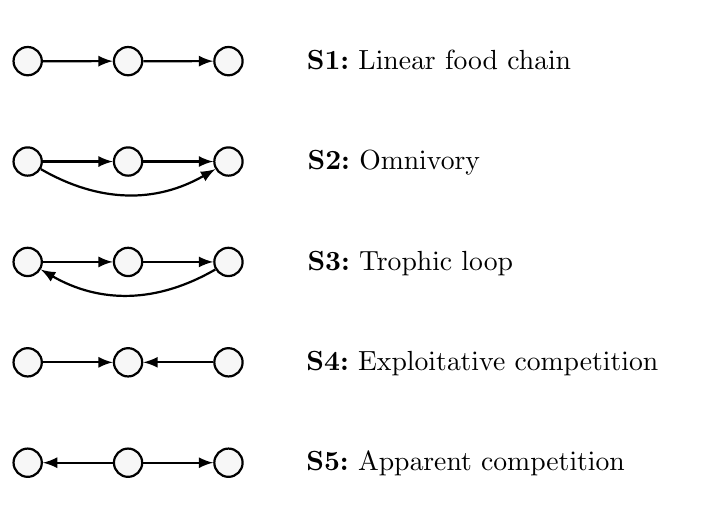
\begin{tikzpicture}[>=latex,text depth=0.25ex,scale=0.85]
		% \draw[help lines] (0,0) grid (10,7);
		\path[use as bounding box] (0,0) rectangle(10,7);
		\tikzstyle{every node}=[draw,minimum size = .3cm,circle,draw=black,fill=black!3]
		\tikzstyle{every path}=[solid,thick]
		
		%% Motif one
		\draw (0,6.5) node (m11) {};
		\draw (1.5,6.5) node (m12) {};
		\draw (3,6.5) node (m13) {};
		\path [->] (m11) edge (m12);
		\path [->] (m12) edge (m13);
		\draw (4,6.5) node [draw = none, fill=none, anchor=west] (lfc) {\textbf{S1:}~Linear food chain};
		
		%% Motif two
		\draw (0,5) node (m21) {};
		\draw (1.5,5) node (m22) {};
		\draw (3,5) node (m23) {};
		\path [->] (m21) edge (m22);
		\path [->] (m22) edge (m23);
		\path [->] (m21) edge [bend right] (m23);
		\draw (4,5) node [draw = none, fill=none, anchor=west] (omn) {\textbf{S2:}~Omnivory};
		
		%% Motif three
		\draw (0,3.5) node (m31) {};
		\draw (1.5,3.5) node (m32) {};
		\draw (3,3.5) node (m33) {};
		\path [->] (m31) edge (m32);
		\path [->] (m32) edge (m33);
		\path [->] (m33) edge [bend left] (m31);
		\draw (4,3.5) node [draw = none, fill=none, anchor=west] (tl) {\textbf{S3:}~Trophic loop};
		
		%% Motif four
		\draw (0,2) node (m41) {};
		\draw (1.5,2) node (m42) {};
		\draw (3,2) node (m43) {};
		\path [->] (m41) edge (m42);
		\path [->] (m43) edge (m42);
		\draw (4,2) node [draw = none, fill=none, anchor=west] (exc) {\textbf{S4:}~Exploitative competition};
		
		%% Motif five
		\draw (0,0.5) node (m51) {};
		\draw (1.5,0.5) node (m52) {};
		\draw (3,0.5) node (m53) {};
		\path [->] (m52) edge (m51);
		\path [->] (m52) edge (m53);
		\draw (4,0.5) node [draw = none, fill=none, anchor=west] (pac) {\textbf{S5:}~Apparent competition};
		
	\end{tikzpicture}
   \caption{The 5 simple-link motifs encompass important scenarios for the flow of biomass across trophic level. Arrows indicates a \emph{feeding} link. Next to each motif is the ecological reality it implies. }
   \label{f:motifDynamics}
\end{figure}

\section{Methods}

\subsection{Data}

We use a collection of 178 community food webs, represented by their adjacency matrix. These food webs were previously published and analyzed by DUNNE, COHEN, and \textcite{Havens1992}. The data were collected by \textcite{Gravel2011a}.

\subsection{A model of biomass dynamics in food webs}

We apply a dynamical model to these food webs. We use an expansion of the classical \textcite{Yodzis1992} model to food webs, such as proposed by \textcite{Brose2006a}. 

\begin{align}
	\frac{dB_{i}}{dt} & = B_{i}\times r\left(1-\frac{B_{i}}{K}\right) - \sum_{j\in\mathrm{consumers}}\frac{x_{j}y_{j}B_{j}F_{ji}}{e_{ji}}\\
	\frac{dB_{i}}{dt} & = -x_{i}B_{i} + \sum_{j\in\mathrm{resources}}x_{i}y_{i}B_{i}F_{ij} - \sum_{j\in\mathrm{consumers}}\frac{x_{j}y_{j}B_{j}F_{ji}}{e_{ji}}
\end{align}

In this model, the extent to which allometric scaling exists in the interaction
strength is regulated by a single parameter $Z$, which represents the body mass
ratio of consumers and their resources. For $Z = 0$, there is no allometric
scaling, and for other values of $Z$, we can explore situations in which
consumers are heavier or lighter than their resources. As in the original model,
we used a value of unity for $r$ and $K$, so that all biomasses are expressed
relatively to the biomass of primary producers. In the formulation of the
original model, we assume that our food webs are made of ectotherm vertebrates
and most of the interactions are carnivory, meaning that the parameter values
are as follows: $e_{ij}$, the assimilation efficiency, is 0.85; $x_{i}$, the
maximum metabolic rate, is equal to $(a_{x}/a_{r})\times(M_{C}/M_{P})^{-0.25}$;
$y_{i}$, the maximal consumption rate, is equal to $a_{y}/a_{x}$; $M = Z^{T}$,
$a_{r} = 1$, $a_{x} = 0.88$, and $y_{i} = 4$.

The functional responses are assumed to be of the predator interference type
(hill exponent $h = 1$, competition coefficient $c = 1$), so that

\begin{equation}
	F_{ij} = \frac{\omega_{ij}B_{j}^h}{B_{0}^{h}+cB_{i}B_{0}^{h}+\sum_{k\in \mathrm{preys}}\omega_{ik}B_{i}^{h}},
\end{equation}

with $B_{0}$ fixed to $1/2$, and $\omega_{ij}$ fixed to $1/n$ wherein $n$ is the
number of preys, to reflect uniform relative consumption rate over consumers,
and no prey preference. For more informations about this model, readers are
encouraged to refer to the original publications
\parencite{Brose2006a,Williams2007}.

In each of the 178 food webs, we simulate this model using 100 replicates of the
following procedure. First, species with a out degree of 0 are primary
producers. Then, we use this information to measure the trophic rank, as the
minimal distance between one species and a primary producer. While other
measures have been used \parencite{Post2002}, this definition makes sense in an
ecosystem functioning perspective, as most of the biodiversity-functioning
relationship appears driven by complementarity in resource use (in addition,
using either the mean or the maximum distance to primary producers yielded
qualitatively similar results). We use the trophic rank information to calculate
the species-specific parameters. At the beginning of each simulation, each
species of the network is assigned a starting population density, drawn
uniformly from $[0.05, 1]$. We let the system run for $10^{4}$ time steps, and
record the individual biomass of each species over the last $10^{3}$ time steps.

\subsection{Analyses}

\paragraph{Network structure}

For each network, we count the number of motifs using the following procedure.
We took all possible groups of three species, and look at the linkage pattern
between them. Motifs are attributed and named as in \textcite{Stouffer2007}. The
total number $N_{m}$ of motifs is counted, and, so as to normalize motif counts
by the network size and connectance, we use the frequency of each motif in the
analyzes, so that for any motif $n$ found $N_{n}$ times,

\begin{equation}
	f(n) = \frac{N_{n}}{N_{m}}.
\end{equation}

This procedure is also done at the level of the species, \emph{i.e.} each time a
species $i$ is found in motif $n$, $N_{n}^{i}$ increases by 1. As for networks,
the motif count of each species is transformed in a frequency, so that if
species $i$ is found in a total of $N_{m}^{i}$ motifs,

\begin{equation}
	f^{i}(n) = \frac{N_{n}^{i}}{N_{m}^{i}}.
\end{equation}

Because of the strong negative linear correlation between the frequency of
motifs S4 and S5 (resp. exploitative and apparent competition), we define a
competition-type ratio, such that

\begin{equation}
	C_{R} = \frac{f(S_4)}{f(S_5)}.
\end{equation}

For values of this ratio larger than unity, there are more exploitative than
apparent competition motifs.

\paragraph{Functioning}

We record the biomass of the whole food web, which we divide by the number of
species $S$, so that

\begin{equation}
	\bar B = \sum_{i=1}^{S}\frac{B_{i}}{S}.
\end{equation}

In addition, the raw biomass of each species is also recorded.

\section{Results}

The 178 networks from our dataset show a large variation in their composition in
the different motifs (Fig.~\ref{f:motifs}). Most of the double-link motifs are
really rare, and because their relevance to energy flow is difficult to
establish, we focus our analysis on the single-link motifs. We present results
at two scales of organization: biomass production for the whole network, and
biomass production for each species within a set of representative networks.

\begin{figure}[tbp]
   \centering
   \begin{tikzpicture}
			\begin{axis}[height=7cm, width=.75\textwidth,
				stack plots=y, enlargelimits=false,
				const plot, area style,
				ymin=0, ymax=1,
				cycle list name=pastel,
				xlabel = Network rank ($\bar B$), ylabel = Motif frequency,
				legend style={
					area legend,
					at={(1.05,0.5)},
					anchor=west,
					legend columns=1}
			]
				\addplot table [x=prank, y=S1] {../w-scaled.dat} \closedcycle;
				\addplot table [x=prank, y=S2] {../w-scaled.dat} \closedcycle;
				\addplot table [x=prank, y=S3] {../w-scaled.dat} \closedcycle;
				\addplot table [x=prank, y=S4] {../w-scaled.dat} \closedcycle;
				\addplot table [x=prank, y=S5] {../w-scaled.dat} \closedcycle;
				\legend{$f(S_{1})$,$f(S_{2})$,$f(S_{3})$,$f(S_{4})$,$f(S_{5})$};
			\end{axis}
		\end{tikzpicture}
		\begin{tikzpicture}
			\begin{axis}[height=7cm, width=.75\textwidth,
				stack plots=y, enlargelimits=false,
				const plot, area style,
				ymin=0, ymax=1,
				cycle list name=pastel,
				xlabel = Network rank ($\bar B$), ylabel = Motif frequency,
				legend style={
					area legend,
					at={(1.05,0.5)},
					anchor=west,
					legend columns=1}
			]
				\addplot table [x=prank, y=S1] {../ep.dat} \closedcycle;
				\addplot table [x=prank, y=S2] {../ep.dat} \closedcycle;
				\addplot table [x=prank, y=S3] {../ep.dat} \closedcycle;
				\addplot table [x=prank, y=S4] {../ep.dat} \closedcycle;
				\addplot table [x=prank, y=S5] {../ep.dat} \closedcycle;
				\legend{$f(S_{1})$,$f(S_{2})$,$f(S_{3})$,$f(S_{4})$,$f(S_{5})$};
			\end{axis}
		\end{tikzpicture}
   \caption{Variation in motif composition across the 178 food webs studied. Networks are ranked on the x-axis as a function of their mean biomass per species at equilibrium. Motif S4 and S5 are the most abundant, and motif S3 is the least abundant. Some double-link motifs are found in the food webs from our dataset, accounting for the small white space atop some bars.}
   \label{f:motifs}
\end{figure}

\paragraph{Biomass production between food webs}

We report patterns of biomass as a function of the composition of each network
in the five single-linked (S1 to S5) motifs (Tab.~\ref{t:ANOVAwebs}). Switching
from scaling ($K = 2$) to no scaling ($K = 0$) has only quantitative differences
on the patterns, with simulations with scaling resulting in a higher mean
biomass. Unless explicitly stated, the figures depict the results of the
simulations with no scaling. Out of the 5 motifs we study, only S5 (apparent
competition) favored biomass production (Fig.~\ref{f:wprod}). The most important
effect on biomass production is the frequency of motif $S_{4}$, either by itself
or when examined as part of the competition type ratio $C_{R}$. Note that using
$C_{R}$ or the additive effect of $S_{4}+S_{5}$ yields the same $R^{2}$. As
$C_{R}$ represents the relative importance of two competition mechanisms, we
will focus on discussing it rather than $S_{4}$ and $S_{5}$ separately.

\begin{table}[tbp]
   \centering
   \topcaption{F-values in the \textsc{anova} explaining mean biomass of all species in the food web, only producers, and only consumers, by the frequency of each motif. All F-values which are not significant ($P \geq 0.05$) are noted as ---. The adjusted $R^{2}$ are given in the last row. \textbf{First rows:} $\bar B \propto f(S_{1}) + f(S_{2}) + f(S_{3}) + f(S_{4}) + f(S_{5})$; \textbf{last rows:} $\bar B \propto f(S_{1}) + f(S_{2}) + f(S_{3}) + \mathrm{log}_{10}C_{R}$.}
   \begin{tabular}{@{} lcccccc @{}}
      \toprule
      & \multicolumn{3}{c}{No scaling} & \multicolumn{3}{c}{Scaling} \\
      \cmidrule(lr){2-4}
      \cmidrule(lr){5-7}
          				& Whole web 		& Producers & Consumers			& Whole web 		& Producers & Consumers\\
      \midrule
      S1				& 3219				& 1352		& 3547				& 2286				& 482		& 3018		\\
      S2				& 540				& 37		& 674				& 685				& 166		& 795		\\
      S3				& 57  				& 8 		& 57 				& 63				& ---		& 54 		\\
      S4				& 12$\times10^{3}$	& 5655		& 10$\times10^{3}$	& 12$\times10^{3}$	& 5637		& 10$\times10^{3}$	\\
      S5				& 29				& 72		& 119 				& 31				& 63		& 125 		\\
      \midrule
      $\mathrm{R}^{2}$	& 0.64 				& 0.44 		& 0.61 				& 0.63 				& 0.41 		& 0.62		\\
      \midrule
      S1				& 3176				& 1317		& 3452				& 2254				& 469		& 2945		\\
      S2				& 532				& 36		& 655				& 676				& 162		& 776		\\
      S3				& 56  				& 8 		& 56 				& 62				& ---		& 53 		\\
      $C_{R}$			& 11$\times10^{3}$	& 5348		& 9629				& 12$\times10^{3}$	& 5297		& 10$\times10^{3}$	\\
      \midrule
      $\mathrm{R}^{2}$	& 0.63 				& 0.43 		& 0.60 				& 0.62		 		& 0.40 		& 0.61		\\
      \bottomrule
   \end{tabular}
   \label{t:ANOVAwebs}
\end{table}

\begin{figure}[tbp]
   \centering
	\begin{tikzpicture}
		\begin{axis}[height=7cm, width=.45\textwidth,
			xmin = 0, xmax = 1, xlabel = Frequency of motif,
			ymin = 0, ymax = 0.8, ylabel = Mean biomass,
			grid=major, name = plot1, cycle list name=hc]
			\addplot+[only marks] table [x=S1,y=bm] {../w-scaled.dat};
			\addlegendentry{$S_{1}$}
			\addplot+[only marks] table [x=S2,y=bm] {../w-scaled.dat};
			\addlegendentry{$S_{2}$}
			\addplot+[only marks] table [x=S4,y=bm] {../w-scaled.dat};
			\addlegendentry{$S_{4}$}
			\addplot+[only marks] table [x=S5,y=bm] {../w-scaled.dat};
			\addlegendentry{$S_{5}$}
		\end{axis}
		\begin{semilogxaxis}[height=7cm, width=.45\textwidth,
			xmin = 0.1, xmax = 10, xlabel= Competition type ratio -- $C_{R}$,
			ymin = 0, ymax = 0.8, ylabel = Mean biomass,
			grid=major, at={($(plot1.east)+(2cm,0)$)},anchor=west,
			cycle list name=hc]
			\addplot+[only marks] table [x=compratio,y=bm] {../w-scaled.dat};
			\addlegendentry{scaling}
			\addplot+[only marks] table [x=compratio,y=bm] {../w-unscaled.dat};
			\addlegendentry{no scaling}
		\end{semilogxaxis}
	\end{tikzpicture}
	\begin{tikzpicture}
		\begin{axis}[height=7cm, width=.45\textwidth,
			xlabel = Frequency of motif,
			ylabel = Mean biomass,
			grid=major, name = plot1, cycle list name=hc]
			\addplot+[only marks] table [x=S1,y=bm] {../ep.dat};
			\addlegendentry{$S_{1}$}
			\addplot+[only marks] table [x=S2,y=bm] {../ep.dat};
			\addlegendentry{$S_{2}$}
			\addplot+[only marks] table [x=S4,y=bm] {../ep.dat};
			\addlegendentry{$S_{4}$}
			\addplot+[only marks] table [x=S5,y=bm] {../ep.dat};
			\addlegendentry{$S_{5}$}
		\end{axis}
		\begin{semilogxaxis}[height=7cm, width=.45\textwidth,
			xlabel= Competition type ratio -- $C_{R}$,
			ylabel = Mean biomass,
			grid=major, at={($(plot1.east)+(2cm,0)$)},anchor=west,
			cycle list name=hc]
			\addplot+[only marks] table [x=compratio,y=bm] {../ep.dat};
			\addlegendentry{scaling}
		\end{semilogxaxis}
	\end{tikzpicture}
   \caption{Mean biomass produced by each species within the 178 food webs. \textbf{Left:} mean biomass expressed as a function of the frequency of the four most important motifs: S1, S2, S4 and S5. Of all the motifs considered here, only the one indicating apparent competition (S5) results in an increase in biomass production. \textbf{Right:} mean biomass expressed as a function of $C_{R}$, with values above unity indicating more exploitative than apparent competition. Simulations with and without allometric scaling yield the same pattern.}
   \label{f:wprod}
\end{figure}

\paragraph{Biomass production within food webs}

\section{Discussion}

%% Main findings
\textbf{FOOD WEB LEVEL}
\begin{itemize}
	\item The frequency of two types of competitions is the most significant effect -- this confirms our result from the PNAS MS than complementarity is the most important mechanism
	\item The frequency of S1 (linear food chains) has a strong impact on consumers, but not producers, biomass -- not sure what it means
	\item Results are not affected by scaling: most of the functioning depends on topology -- good thing, because it means we need much less information to predict functioning than if allometry is important (also worth noting, the patterns here are exactly the same as with my previous extremely simple Lotka-Volterra model)
\end{itemize}

\printbibliography


\end{document}  
